\documentclass[landscape]{exam}

\usepackage{2in1, lscape} 
\usepackage{units} 
\usepackage[fleqn]{amsmath}
\usepackage{float}
\usepackage{mdwlist}
\usepackage{booktabs}
\usepackage{caption}
\usepackage{fullpage}
\usepackage{enumerate}
\usepackage{graphicx}
\usepackage{parskip}

\printanswers

\everymath{\displaystyle}

\printanswers

\title{Statistics \\ Week Ten}
\date{\today}
\author{}

\begin{document}

  \maketitle
  \tableofcontents

  \section{Tea/Milk Experiment}

  \subsection{History}
  \begin{itemize*}
    \item determine if subject can tell whether tea was made milk/tea or tea/milk.

    \item party in 1920 in Cambridge

    \item According to second-hand testimony, woman told them apart flawlessly

  \end{itemize*}

  \subsection{Terminology}
  \begin{description*}
    \item[treatment] thing you are trying to find out (adding cream first)
    \item[control] no change (usual order)
    \item[factor] tea/milk order
  \end{description*}

  \subsection{One Trial Experiment}
  With 2 cup experiment, subject has 50\% of success by chance.

  With 4 cup experiment:
  \begin{itemize*}
    \item $4 \times 3 = 12$ ways to choose 2 cups.  

    \item $2 \times 1 = 2$ 2 ways to arrange two identical cups, so 2 copies of
      each selection ($a_1a_2b_1b_2$ and $a_2a_1b_2b_1$ are identical)

    \item 6 unique ways to choose 2 out of 4. aabb, abab, abba, bbaa,
      baba, baab.
    \item random guess would be correct 1 out of 6 or 17\% of the time
  \end{itemize*}

  With 6 cup experiment:
  \begin{itemize*}
    \item $6 \times 5 \times 4 = 120$ ways to choose 3 cups.  
    \item $3 \times 2 \times 1 = 6$ copies of each arrangement
    \item random guess would be correct 1 out 20 or 5\% of the time
  \end{itemize*}

  With 8 cup experiment:
  \begin{itemize*}
    \item $8 \times 7 \times 6 \times 5 = 1680$ ways to choose 4 cups.  
    \item $4 \times 3 \times 2 \times 1 = 24$ copies of each arrangement
    \item random guess would be correct 1 out of 70 or 1.4\% of the time
  \end{itemize*}

  With 10 cup experiment:
  \begin{itemize*}
    \item $10 \times 9 \times 8 \times 7 \times 6 = 30240$ ways to choose 5 cups.  
    \item $5 \times 4 \times 3 \times 2 \times 1 = 120$ copies of each arrangement
    \item random guess would be correct 1 out of 252 or 0.4\% of the time
  \end{itemize*}

  \begin{itemize*}
    \item with any number of cups, there is always at least a tiny chance of
      success by chance
    \item usual definition of ``statistically significant'' is experiment where
      random guess would be successful less than 5\% of the time
    \item you need to identify possible outcomes and chance of each before the
      experiment starts so you design experiment that will answer question to
      your satisfaction
  \end{itemize*}

  \subsection{Perfection Not Required}
  If taster can only usually but not always tell the difference, you could
  define success as 3 out of 4 right in an 8 cup experiment.

  \begin{itemize*}
    \item 1 way to get 4 out of 4
    \item 4 ways to pick a cup from set A to get wrong and 4 cups to choose swap
      it with from set B: 16 ways to get one cup wrong
    \item random guess would be correct 17 out of 70 or 24\% of the time.  You
      could say with 76\% confidence that person can tell difference
  \end{itemize*}

  To get back to 95\% confidence, expand trial to 12 cups and count either 5 or
  6 correct as success:

  6 out of 6:
  \begin{itemize*}
    \item $12 \times 11 \times 10 \times 9 \times 8 \times 7 = 665,280$ ways to
      choose 6 cups.  
    \item $6 \times 5 \times 4 \times 3 \times 2 \times 1 = 720$ duplicates
    \item random guess would be correct 1 out of 924 or 0.1\% of the time
  \end{itemize*}

  5 out of 6:
  \begin{itemize*}
    \item 6 ways to get wrong cup from set A and 6 choices of cup to swap with
      in set B: 36 ways to get exactly one cup wrong
    \item random guess would be correct (at least 5 out of 6 right) $36 + 1 =
      37$ out of 924 or 4\% of the time
  \end{itemize*}

  Other approaches
  \begin{itemize*}
    \item With 10 8 cup trials, where success is 3 out of 4, chance of 6 out of
      10 successes by chance (3 out of 4 cups identified correctly) is 1.7\%
      
    \item With 10 8 cup trials where success is perfect 4 out of 4, chance of
      getting 2 perfect scores by chance in 10 attempts is only 0.85\%
  \end{itemize*}

  2 out of 4 is too easy: 17 ways to get at least 3 wrong, $70 - 17 = 53$ ways
  to get at least 2 right.  Chance of at least 2 by chance is 53 out of 70 or
  76\%.

  \subsection{Randomization}
  Try to minimize differences other than tea/milk order.

  One approach is to try to identify everything: cup color, weight, temperature,
  etc. and then try hard to make sure each treatment matches in all other
  variables.  It's impossible to know everything that might matter, so this
  approach is problematic.

  Another approach is to do everything except for thing that matters (tea/milk
  order) randomly.  Any chance variation while average out.

  Of course, randomization won't help if there is some dramatic difference, like
  two kinds of tea (Irish Breakfast and English Breakfast, for example).  If you
  can't narrow it down to one kind of tea, you should consider a {\em block}
  design, where you experiment separately on each block (tea type).

  Randomization won't help if there is some huge difference like sugar in the
  bottom of some of the cups.

  \section{Agriculture}
  \begin{itemize*}
    \item before Fisher, agriculture experiments ad-hoc mixture of formulas
      which tried to account for variations in soil, weather, seeds, etc.

    \item Fisher introduced randomization of everything other than what was
      being measured.

    \item There was considerable debate with other researchers.  Some
      researchers thought that the best results were achieved by explicitly
      accounting for everything that mattered.  Fisher thought you couldn't
      possibly think of everything that mattered, and it was cheaper, easier,
      and more effective to acknowledge this and use randomization.

    \item with 3 treatments and control:
      \begin{enumerate*}
        \item divide single plot into 4 quadrants.  problem is that one quadrant
          may have better soil than another
        \item divide each quadrant into 4 quadrants (16 plots in all) and plant
          all 4 variations in each quadrant
        \item use ``Latin Square.'' Each row has one of the treatments and each
          column has one of the treatments.  Like soduku.
      \end{enumerate*}
  \end{itemize*}

  \section{Salk Polio Vaccine}
  \subsection{History}
  \begin{itemize*}
    \item 1916-54, thousands of cases
    \item 1954 trial of new Jonas Salk vaccine for polio
    \item Polio affects richer kids more than poorer kids. Poorer kids tend to
      be exposed to polio early in life and get very mild cases which allows
      them to develop immunity.
    \item parental permission required for vaccination
    \item richer parents were more likely to give permission for vaccination
    \item disease spreads through proximity with other people with the disease
    \item vaccine looked promising but it was uncertain whether it would
      actually help or possibly hurt
  \end{itemize*}

  \subsection{Original Design}
  The original design was to vaccinate all grade 2 kids whose parents would
  consent, leaving grades 3 and 4 kids as controls.  This would allow any second
  grader who wanted the vaccine to get it.

  problems:
  \begin{itemize}

    \item Parents who consented likely to be richer than parents who didn't.
      This biased the study against the vaccine since the polio rate is higher
      among this group.

    \item Disease was spread through contact.  Since kids tend to hang out with
      their own grade level, the incidence of the disease in a particular grade
      level was likely to be different from the incidence of the disease in the
      other grade levels. This might bias the study for or against the vaccine,
      based on chance.
  \end{itemize}

  Problem: both of these problems are that the control group is different from the
  treatment group.

  Solution: treatment and control have to be drawn from the same population

  \subsection{Final Design}
  Another problem was how to make the treatment and control groups similar.  One
  option would be to look at all the characteristics of the kids (race, income,
  gender, health, number of friends, etc.) and try to get similar kids in each
  group (stratified sample).  Since it was hard to identify everything that
  might matter, they used a simple random sample.

  \begin{itemize*}
    \item 2 million kids
    \item 500,000 vaccinated (treatment)
    \item 500,000 selected for vaccination but declined to participate
    \item 1,000,000 unvaccinated (controls)
  \end{itemize*}

  \section{Breast Cancer Study}
  Health Insurance Plan of NY (HIP) study in 1963.

  Conclusions:
  \begin{itemize*}
    \item screening didn't affect diseases other than breast cancer
    \item poor less likely to accept screening
    \item most diseases other than breast cancer affect poor more than rich
  \end{itemize*}

  \begin{table}
    \centering
    \begin{tabular}{lrrrrr}
      & & \multicolumn{2}{c}{Breast Cancer} & \multicolumn{2}{c}{All Other} \\
                               \cmidrule(r){3-4} \cmidrule(r){5-6}    
                      &        & number & rate & number & rate \\
      Treatment group \\
      examined        & 20,200 & 23     & 1.1  & 428    & 21 \\
      refused         & 10,800 & 16     & 1.5  & 409    & 38 \\
      total           & 31,000 & 39     & 1.3  & 837    & 27 \\
    \midrule
      control group   & 31,000 & 63     & 2.0  & 879    & 28 \\
    \end{tabular}
    \caption{Breast cancer study: cause of death}
    \label{tab:breast.cancer}
  \end{table}

  \begin{itemize*}
    \item does screening save lives?
    \item why is rate for ``all other'' same for treatment and control groups?
    \item why is rate for all other causes higher for ``refused'' than
      ``examined'' groups?

    \item breast cancer affects rich more than poor.  which numbers confirm
      this?

      \begin{solution}
        Rich people tend to accept.  Income of groups, in order, is examined,
        control, refused, since control has mix of rich and poor and
        examined/refused are segregated by income.  Death rate among control
        group is higher than death rate among refused, and only thing different
        is income.
      \end{solution}

    \item death rate (all causes) among accepted is about half death rate among
      refused.  Did screening cut the death rate in half?  What explains the
      difference in death rate?

    \item Is comparing accepted vs. refused a fair comparison?  Is it biased for
      or against screening?

      \begin{solution}
        Since the people who accepted the screening tend to have more money, and
        money is positively correlated with breast cancer incidence, this
        comparison would be biased against screening.
      \end{solution}

    \item Someone claims that encouraging women to come in for breast cancer
      screening encourages their health conciousness so they live longer for
      that reason.  Is the data consistent or inconsistent with that claim?

      \begin{solution}
        Inconsistent.  The only thing affected by the screening is the breast
        cancer rate.
      \end{solution}

    \item In the first year of the study, 67 breast cancers were found in the
      ``examined'' group, 12 in the refused group, and 58 in the control group.
      True or false: screening causes breast cancer.

      \begin{solution}
        Comparing raw numbers doesn't make sense, since there are different
        numbers in each group.  It makes more sense to look at the percentages
        with cancer detected in each group:
        \begin{itemize*}
          \item examined: 0.33\%
          \item refused: 0.11\%
          \item control: 0.19\%
        \end{itemize*}

        More cancer is detected among the examined because:
        \begin{itemize*}
          \item they have more money, so they are more likely to get breast
            cancer
          \item the regular exams detect cases that go undetected in the other
            groups
        \end{itemize*}

        Control has more than refused because control is slightly richer.
      \end{solution}

  \end{itemize*}

  \section{Placebo Effect}

  Drug trial for headache remedy.

  \begin{tabular}[H]{rcccc}
    \toprule
    group & week 1 & week 2 & week 3 & week 4 \\
    \midrule
    I     & A      & B      & C      & D \\
    II    & B      & A      & D      & C \\
    III   & C      & D      & A      & B \\
    IV    & D      & C      & B      & A \\
  \end{tabular}

  success rate:
  \begin{tabular}[H]{cccc}
    \toprule
    A  & B  & C  & D \\
    \midrule
    84 & 80 & 80 & 52 \\
    \bottomrule
  \end{tabular}

  D was the placebo, so its success was surprising.  A was the combination of B
  and C.

  \begin{figure}[H]
    \centering
    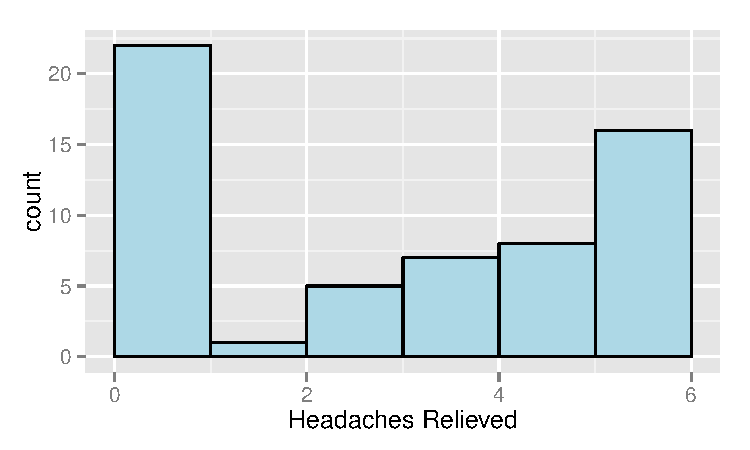
\includegraphics{figures/placebo.pdf}
    \caption{Placebo Effect}
    \label{fig:placebo}
  \end{figure}

  Why is Latin Square better than:
  \begin{tabular}[H]{rcccc}
    \toprule
    group & week 1 & week 2 & week 3 & week 4 \\
    \midrule
    I     & A      & B      & C      & D \\
    II    & A      & B      & C      & D \\
    III   & A      & B      & C      & D \\
    IV    & A      & B      & C      & D \\
  \end{tabular}
\end{document}

